\section{NX Flow}
\label{sec:nxflow}
%
%
NX\texttrademark~Flow is a commercial software part of the Simcenter\texttrademark~solution portfolio~\cite{nxflow}. It is developed at Maya Heat Transfer Technologies in Montreal. The program has the following characteristics:
\begin{itemize}
    \item Dimensional
    \item Unstructured
    \item Vertex-centered
    \item Uses a control-volume based finite element (CVFE) method
    \item Pressure-based
\end{itemize}
The mesh structure is explained in~\Cref{sec:nxmesh}, an overview of the CVFE method is given in~\Cref{sec:cvfem}, the characteristics of a pressure-based code are given in~\Cref{sec:pbased}, the discretization is described in~\Cref{sec:nxnum} and wall distance calculation methods are presented in~\Cref{sec:nxwalldist}.
%
\subsection{Computational grid}
\label{sec:nxmesh}
%
As opposed to syn3D, NX Flow solves the governing equations on a computational domain tessellated with unstructured grids of various element types.. This allows for greater flexibility in adapting the grid to arbitrarily complex domains. The grids are typically composed of hexahedrons and tetrahedrals, although pyramids and wedges are also often used as transition elements. Thus, significant bookkeeping is required in order to keep track of the connectivity compared to structured grids. The reader is referred to~\cite{blazek2015computational} for a more detailed discussion on unstructured grids.

Another difference between syn3D and NX Flow is that the latter locates the field points at the vertices, not the element centroids, making it a vertex-centered, or cell-vertex, code. However, it still is a finite volume code, which raises the question of how the CVs are constructed. This is done by generating a so-called dual mesh, which is similar to the auxiliary CV construction in syn3D as described in~\Cref{sec:synns}. In two dimensions, as depicted in~\Cref{fig:dualmeshtwo}, a CV is constructed around a given vertex by looping over the edges containing the vertex and joining the midpoints of those edges to the face centers. Using finite volume terminology, these lines (one-dimensional surfaces) are referred to as \textit{integration surfaces}. It goes without saying that distinguishing between a control volume and an element is crucial. One speaks of a CV sector or element sector when referring to the portion of a CV contained in a single element. It can also be said that a given element is divided into $N$ sectors, where $N$ is the number of vertices, or nodes, this element is made up of.
\begin{figure}
    \centering
    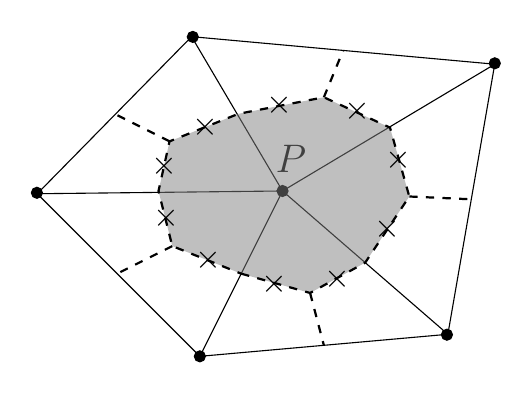
\begin{tikzpicture}[scale=3.5]
    %   % Generated with mktridual.py
\draw[] (0.00,0.00) -- (0.90,0.08) -- (1.07,1.06) -- (-0.03,1.16) -- (-0.59,0.59) -- cycle;
\draw [fill] (0.0, 0.0) circle [radius=0.02] node [] {};
\draw [fill] (0.896575228282571, 0.07844016847289235) circle [radius=0.02] node [] {};
\draw [fill] (1.0702234059495015, 1.0632479214851003) circle [radius=0.02] node [] {};
\draw [fill] (-0.025590761951418628, 1.1591192385075249) circle [radius=0.02] node [] {};
\draw [fill] (-0.5912761869006568, 0.5934338135582868) circle [radius=0.02] node [] {};
\draw [fill] (0.3, 0.6) circle [radius=0.02] node [above=3pt,xshift=3pt] {\Large $P$};
\draw[] (0.30,0.60) -- (0.00,0.00);
\draw[] (0.30,0.60) -- (0.90,0.08);
\draw[] (0.30,0.60) -- (1.07,1.06);
\draw[] (0.30,0.60) -- (-0.03,1.16);
\draw[] (0.30,0.60) -- (-0.59,0.59);
\draw[dashed,thick] (0.40,0.23) -- (0.45,0.04);
\draw[dashed,thick] (0.76,0.58) -- (0.98,0.57);
\draw[dashed,thick] (0.45,0.94) -- (0.52,1.11);
\draw[dashed,thick] (-0.11,0.78) -- (-0.31,0.88);
\draw[dashed,thick] (-0.10,0.40) -- (-0.30,0.30);
\draw[fill=gray,fill opacity=0.5,dashed,thick] (0.15,0.30) -- (0.40,0.23) -- (0.60,0.34) -- (0.76,0.58) -- (0.69,0.83) -- (0.45,0.94) -- (0.14,0.88) -- (-0.11,0.78) -- (-0.15,0.60) -- (-0.10,0.40) -- (0.15,0.30);
\node at (0.27,0.26) {\large $\times$};
\node at (0.50,0.28) {\large $\times$};
\node at (0.68,0.46) {\large $\times$};
\node at (0.72,0.71) {\large $\times$};
\node at (0.57,0.89) {\large $\times$};
\node at (0.29,0.91) {\large $\times$};
\node at (0.02,0.83) {\large $\times$};
\node at (-0.13,0.69) {\large $\times$};
\node at (-0.12,0.50) {\large $\times$};
\node at (0.03,0.35) {\large $\times$};

% \node [align=left] at (0.0, -0.3) {
%     \begin{tabular}{cl}
%     $\times$ & Integration point\\
%     \tikz\draw[fill] circle (0.5ex); & Field point
%     \end{tabular}  
% };
    \end{tikzpicture}
    \caption{Dual control volume of a cell-vertex scheme in two dimensions. Integration surfaces are shown as dashed lines, the CV around $P$ is filled in gray, elements are separated by solid lines, the field point is shown as a solid black circle and integration points are shown as crosses.}
    \label{fig:dualmeshtwo}
\end{figure}

In three dimensions, sectors are generated by joining the element centroid to the element face centers, in combination with lines joining element face centers to the mid-points of the element edges. Again, the sub-division of an element yields as many sectors as vertices on the element.

The terminology introduced here will be used for the remainder of this work of~\Cref{sec:nxflow}. It should also be noted that ``vertex'' and ``node'' are used interchangeably.

\subsection{Control-volume based finite element method}
\label{sec:cvfem}
%
The CVFE method was first proposed by Baliga and Patankar in~\cite{baliga1980new,baliga1983control}. This new method borrows two characteristics from the finite element method (FEM):
\begin{enumerate}
    \item the use of element-based linear Lagrangian interpolation functions (shape functions)
    \item an element-by-element compilation of the coefficients in the discretized equations
\end{enumerate}
These two characteristics are briefly discussed in the following sections. Readers interested in a thorough discussion of the classical FEM applied to fluid flow problems are referred to~\cite{reddy2000finite}.

\subsubsection{Shape functions}
The shape functions $\shape$ represent the variation of solution inside an element. This allows one to calculate the value of a field variable $\phi$ at an $(s,t,u)$ coordinate within the element as follows:
\begin{equation*}
    \phi(s, t, u) = \sum_n^N \shape(s, t, u)_n\phi_n,
\end{equation*}
\begin{figure}
    \centering
    \begin{tikzpicture}[scale=4.0]
    %   \draw [fill] (0.0, 0.0) circle [radius=0.01] node [below] {1};
\draw [fill] (1.0, 0.0) circle [radius=0.01] node [below] {2};
\draw [fill] (1.0, 1.0) circle [radius=0.01] node [above] {3};
\draw [fill] (0.0, 1.0) circle [radius=0.01] node [above] {4};
\draw[dashed] (0.50,0.00) -- (0.50,0.50);
\node at (0.50,0.25) { $\times$};
\draw[dashed] (1.00,0.50) -- (0.50,0.50);
\node at (0.75,0.50) { $\times$};
\draw[dashed] (0.50,1.00) -- (0.50,0.50);
\node at (0.50,0.75) { $\times$};
\draw[dashed] (0.00,0.50) -- (0.50,0.50);
\node at (0.25,0.50) { $\times$};
\draw[] (0.00,0.00) -- (1.00,0.00) -- (1.00,1.00) -- (0.00,1.00) -- cycle;
\draw [thick, <->] (0.20,0.00) node [below right] {$s$} -- (0.00,0.00) -- (0.00,0.20) node [left] {$t$};
\draw [very thick, ->] (1.3, 0.5) -- (1.7, 0.5);
\draw [fill] (2.0, 0.0) circle [radius=0.01] node [below] {1};
\draw [fill] (2.8, 0.0) circle [radius=0.01] node [below] {2};
\draw [fill] (2.9, 1.1) circle [radius=0.01] node [above] {3};
\draw [fill] (2.05, 1.0) circle [radius=0.01] node [above] {4};
\draw[dashed] (2.40,0.00) -- (2.44,0.53);
\node at (2.42,0.26) { $\times$};
\draw[dashed] (2.85,0.55) -- (2.44,0.53);
\node at (2.64,0.54) { $\times$};
\draw[dashed] (2.47,1.05) -- (2.44,0.53);
\node at (2.46,0.79) { $\times$};
\draw[dashed] (2.02,0.50) -- (2.44,0.53);
\node at (2.23,0.51) { $\times$};
\draw[] (2.00,0.00) -- (2.80,0.00) -- (2.90,1.10) -- (2.05,1.00) -- cycle;
\draw [thick, <->] (2.16,0.00) node [below right] {$s$} -- (2.00,0.00) -- (2.01,0.20) node [left] {$t$};

    \end{tikzpicture}
    \caption{General linear quadrilateral element (right) and its representation in the natural coordinate system (left)}
    \label{fig:naturalcsys}
\end{figure}
where $N$ is the number of nodes in the element, $\phi_n$ is the stored value of $\phi$ at node $n$. The $s,t,u$ coordinate system is local to each element and is also referred to as the natural coordinate system in the FEM literature. Construction of shape functions in the $x,y,z$ coordinate system results in complex algebraic expressions, which is why it is best to express them in terms of the natural coordinates. Moreover, the integration point locations for a given element type will always be at the same $s,t,u$ coordinates. Values of $s,t,u$ are only allowed to vary between 0 and 1. The natural coordinate system transformation is illustrated in~\Cref{fig:naturalcsys} for a quadrilateral element (two-dimensional). For such an element, the shape functions can be written as:
\begin{align*}
    \shape_1(s,t) &= (1-s)(1-t)\\
    \shape_2(s,t) &= s(1-t)\\
    \shape_3(s,t) &= st\\
    \shape_4(s,t) &= (1-s)t.
\end{align*}
It is then straightforward to obtain the shape function derivatives with respect to local coordinates, which are given by:
\begin{equation*}
    \pdiff{\phi}{s_i} = \sum_n^N \pdiff{\shape_n}{s_i}\phi_n,
\end{equation*}
where $s_i$ represents the $i$-th component in the natural coordinate system.

Similarly to the generalized curvilinear coordinates, a transformation is necessary to calculate the shape function derivatives with respect to the global coordinates $x,y,z$. The position vector can be expressed as a function of the $s,t,u$ coordinates as:
\begin{equation*}
    \vec{x}(s,t,u) = \sum_n^N \shape(s,t,u)_n\vec{x}_n.
\end{equation*}
This leads to the following metric formulation:
\begin{equation}
    \left.\pdiff{\vec{x}}{s_j}\right|_{(s,t,u)} =
        \sum_n^N \left(\left.\pdiff{\shape_n}{s_j}\right|_{(s,t,u)} \vec{x}_{n}\right).
\end{equation}

The derivatives of $\phi$ with respect to the natural coordinates can be written in the following matrix form using the chain rule:
\begin{equation*}
    \begin{pmatrix}
        \pdiff{x}{s} & \pdiff{y}{s} & \pdiff{z}{s} \\
        \pdiff{x}{t} & \pdiff{y}{t} & \pdiff{z}{t} \\
        \pdiff{x}{u} & \pdiff{y}{u} & \pdiff{z}{u}
    \end{pmatrix}
    \begin{bmatrix}
        \pdiff{\phi}{x} \\
        \pdiff{\phi}{y} \\
        \pdiff{\phi}{z}
    \end{bmatrix}
    =
    \begin{bmatrix}
        \pdiff{\phi}{s} \\
        \pdiff{\phi}{t} \\
        \pdiff{\phi}{u}
    \end{bmatrix}.
\end{equation*}
This system can be numerically inverted using Kramer's rule.
The derivative $\partial \phi/\partial x$ at an integration point in the element can then be written as:
\begin{equation*}
    \left.\pdiff{\phi}{x_i}\right|_{ip} = \sum_n^N \left.\pdiff{\shape_n}{x_i}\right|_{ip}\phi_n.
\end{equation*}
It should be noted that the evaluation of $\phi$ and its derivative inside an element can be computed with second-order accuracy regardless of the shape of the element, which is a significant advantage of using this method -- the approximations in~\Cref{sec:syn3d} are at most second-order accurate, depending on the skewness and orthogonality of the grid.


\subsubsection{Compilation of the coefficients}
The CVFE method uses the integral form of the equations as discussed in~\Cref{sec:fv}, and fluxes through the integration surfaces around a control volume must be evaluated. Due to the dual mesh configuration, the integration surfaces as well as the integration points lie completely inside the elements. The surface integrals can then be calculated element-wise and accumulated to each control volume appropriately. The surface integrals are then guaranteed to be conservative. Moreover, because of the way the shape functions are constructed, the value of the flux at a given integration point depends on the field variables at all nodes in that element, regardless of whether the integration point belongs to their control volume. In other words, the stencil involved in the computation of a flux always includes all the vertices of the element in which the flux is computed.

It should be noted that boundaries of the domain require special treatment, since the surfaces are not located inside any element. This is discussed further below.

\subsection{Pressure-based solver}
\label{sec:pbased}
The main difference between a density-based and a pressure-based solver is the dependent variable in the mass equation, which is density in the former and pressure in the latter. Because a large portion of users of NX Flow want to simulate flows involving liquids, which have a constant density, the developers of NX Flow chose the pressure-based approach. In the case of ideal gases, the density is updated using the ideal gas law at each iteration.

NX Flow employs the collocated variables approach, i.e. pressure and velocity are stored at the same locations, proposed by Rhie and Chow~\cite{rhie1983numerical} in order to avoid pressure checkerboarding.

\subsection{Discretization of the governing equations}
\label{sec:nxnum}
This section describes the numerical discretization of the terms in the mass, momentum, energy and turbulence equations.

NX Flow being a commercial code, offers a wide variety of options to its users. For the sake of conciseness, only the options used to solve the problems in this work are described.

\subsubsection{Temporal discretization}
NX Flow uses the fully-implicit first-order backward Euler approach to discretize the time derivative of all partial differential equations. It solves the mass and momentum equations together, which yields an updated pressure and velocity field.

%In the case of the conservation laws, this leads to a coupled system of five equations for each control volume:
%\begin{equation*}
%    \left[
%        \frac{V}{\Delta t^n} - \pdiff{\vec{R}^n}{\vec{W}}
%    \right] \Delta \vec{W}^n = \vec{R}^n
%\end{equation*}
%where $\vec{W}$ is defined in~\Cref{eq:wstate}.

The turbulence and energy equations are not coupled with the mass and momentum equations; they are solved separately in a segregated manner. The linear systems are solved using an iterative solver such as GMRES.

\subsubsection{Discretization of convective fluxes}
The convective flux of an arbitrary quantity over an integration surface can be written in the following general form:
\begin{equation*}
    \int_S (\rho\vec{u}\phi)\cdot\vec{n}~dS = \dot{m}_{ip}\phi_{ip},
\end{equation*}
where $\dot{m}_{ip}$ is the mass flow rate through the integration surface and is evaluated using the shape functions along with a pressure correction term~\cite{schneider1987control,rhie1983numerical}. The method is actually slightly modified from the cited references, but cannot be discussed.

The value of $\phi$ at the integration point also needs to be approximated in terms of the nodal values of $\phi$. The default scheme for this is a first-order upwind scheme, in which $\phi_{ip}$ is approximated by the value of $\phi$ at the upstream node, i.e.:
\begin{equation*}
    \phi_{ip} = \phi_{i},
\end{equation*}
where the upstream node is determined using the sign of the mass flux. This scheme leads to a stable and quick convergence at the expense of reduced accuracy.

\subsubsection{Discretization of viscous fluxes}
Computation of the diffusive fluxes requires evaluation of the diffusion coefficient and spatial derivatives at the integration points. This is simply done using the finite element shape functions. The gradient and diffusion coefficient at an integration point are then evaluated as:
\begin{align*}
    \Gamma_{ip} &= \sum_n^N \left.\shape_n\right|_{ip}\Gamma_n \\
    \left.\nabla\phi\right|_{ip} &= \sum_n^N \left.\nabla\shape_n\right|_{ip}\phi_n.
\end{align*}

\subsubsection{Discretization of pressure term}
The pressure gradient term is treated as a surface force via the divergence theorem, similarly to syn3D. The value of pressure must then be evaluated at all integration points, which is done using the shape functions.

\subsubsection{Discretization of nodal gradients}
Source terms sometimes require the computation of gradients at field points, as opposed to at an integration point. Such nodal gradients can also be computed using a form of the divergence theorem. The gradient of $\phi$ at node $P$ can then be computed as follows:
\begin{equation*}
    (\nabla \phi)_P = \frac{1}{V}\sum_{ip}(\phi\vec{n})_{ip}.
\end{equation*}
The formula requires that $\phi$ be evaluated at integration points, which is done using the shape functions.

\subsubsection{Boundary conditions}
NX Flow was unfortunately not developed with external flows in mind and does not offer far-field boundary conditions in its catalogue. The user must then use internal flow BCs such as inlets and openings. The following boundary conditions are used in this work:
\begin{itemize}
    \item Solid wall
    \item Inlet
    \item Opening
    \item Symmetry plane
\end{itemize}
Treatment of boundary conditions in a vertex-centered code is quite different from that of a cell-centered code since some field points may lie on the boundary, as depicted in~\Cref{fig:cvfebc}. Such points have integration surfaces corresponding to segments of the boundary. It should be noted that evaluation of fluxes over the domain then requires two loops: one over the elements and the interior integration surfaces as well as one over the boundary integration surfaces.
\begin{figure}
    \centering
    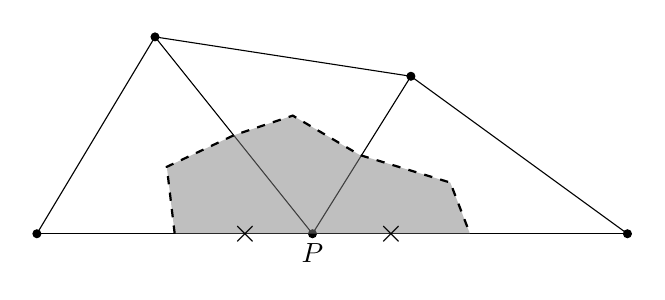
\begin{tikzpicture}[scale=5.0]
    %   \draw[thin] (-1.00,0.00) -- (1.00,0.00);
\draw [fill] (-0.7, 0.0) circle [radius=0.01] node [] {};
\draw [fill] (0.0, 0.0) circle [radius=0.01] node [below] {$P$};
\draw [fill] (0.8, 0.0) circle [radius=0.01] node [] {};
\draw [fill] (-0.4, 0.5) circle [radius=0.01] node [] {};
\draw [fill] (0.25, 0.4) circle [radius=0.01] node [] {};
\draw[] (-0.70,0.00) -- (0.00,0.00);
\draw[] (-0.70,0.00) -- (-0.40,0.50);
\draw[] (0.00,0.00) -- (0.80,0.00);
\draw[] (0.00,0.00) -- (-0.40,0.50);
\draw[] (0.00,0.00) -- (0.25,0.40);
\draw[] (0.80,0.00) -- (0.25,0.40);
\draw[] (-0.40,0.50) -- (0.25,0.40);
\draw[fill=gray,opacity=0.5,draw=none] (-0.35,0.00) -- (-0.37,0.17) -- (-0.20,0.25) -- (-0.05,0.30) -- (0.12,0.20) -- (0.35,0.13) -- (0.40,0.00) -- cycle;
\draw[dashed,thick] (-0.35,0.00) -- (-0.37,0.17) -- (-0.20,0.25) -- (-0.05,0.30) -- (0.12,0.20) -- (0.35,0.13) -- (0.40,0.00);
\node at (-0.17,0.00) {\large $\times$};
\node at (0.20,0.00) {\large $\times$};
    \end{tikzpicture}
    \caption{Control volume for a boundary vertex $P$. Only boundary integration points are shown.}
    \label{fig:cvfebc}
\end{figure}

Symmetry planes require that there be no flux through the boundary. The implementation of such a boundary condition simply requires not calculating any fluxes through the boundary integration surfaces.

In an inlet BC, the user specifies values for velocity and its direction as well as pressure, temperature and turbulence quantities. Since the integration point is on the boundary, convective and diffusive fluxes can be calculated using the user-specified values as the $ip$ values, i.e. no interpolation is required. The gradients are calculated using the shape function derivatives, except that the node values are replaced with the integration point values for nodes on the boundary. The gradient of $\phi$ at a boundary integration point $ip,b$ can then be expressed as a sum over the interior nodes, the ones not on a boundary, and boundary nodes:
\begin{equation*}
    \left.\nabla\phi\right|_{ip,b} = \sum_{interior}\left.
        \nabla\shape_n\right|_{ip,b}
    \phi_n + \sum_{boundary}\left.
        \nabla\shape_n\right|_{ip,b}
    \phi_{ip,b}.
\end{equation*}

Opening BCs specify pressure, temperature and turbulence quantities. The velocity at boundary integration points is obtained by shape function interpolation, which determines whether the opening is an inflow or outflow. The advection term requires no special treatment. On the other hand, the diffusion flux is only calculated if the flow is outgoing. All openings used in this work should be treated as outflows.

Viscous wall boundary conditions can be implemented strongly by directly imposing prescribed values at the nodes (Dirichlet) or weakly by instead imposing a condition on the flux through specification of $\phi_{ip,b}$. A detailed discussion can be found in~\cite{nordstrom2012weak}. This BC is currently implemented weakly for the mass and momentum and strongly for the turbulence equations.

\subsection{Wall distance calculation}
\label{sec:nxwalldist}
NX Flow also offers both the brute force approach and Poisson approach to calculate the wall distance. The brute force approach finds the nearest node for every field point, and the Poisson equation is solved with the finite volume method, exactly like the Navier-Stokes equations.